\documentclass[12pt,a4paper,oneside,titlepage] {article}

\usepackage[T2A]{fontenc}
\usepackage[utf8]{inputenc}
\usepackage[russian]{babel}
\usepackage{hyperref}
\usepackage{multicol}
\usepackage{listings}
\usepackage{geometry}
\usepackage{minted}

\usepackage{graphicx}
\graphicspath{ {./images/} }
\usepackage{wrapfig}

\begin{document}

% НАЧАЛО ТИТУЛЬНОГО ЛИСТА
\begin{center}
  \hfill 
  \break
  \textbf{
    \footnotesize{Министерство науки и высшего образования Российской Федерации}\\
    \hfill \break
    \footnotesize{Федеральное государственное бюджетное образовательное учреждение высшего образования}\\
    \small{«МОСКОВСКИЙ ГОСУДАРСТВЕННЫЙ ТЕХНИЧЕСКИЙ УНИВЕРСИТЕТ имени Н.Э.БАУМАНА\\(национальный исследовательский университет)»}}\\
    \footnotesize{(МГТУ им. Н.Э. Баумана)}\\
    \includegraphics[width=25mm,scale=0.25]{emblem}
\end{center}
\hfill 
\break
\normalsize{Факультет: Информатика и системы управления}\\
\hfill \break
\normalsize{Кафедра: Теоретическая информатика и компьютерные технологии}\\
\hfill\break
\begin{center}
  \textbf{\large{Лабораторная работа №2}}\\
  \large{Реализация простейшего класса на языке программирования \bfseries{Java}}\\
\end{center}
\hfill \break
\hfill \break
\hfill \break
\begin{flushright}
  \normalsize{
    Выполнил\\
    студент группы ИУ9-11Б\\
    Лисов Алексей
  }
\end{flushright}
\hfill \break
\hfill \break
\hfill \break
\hfill \break
\hfill \break
\hfill \break

\begin{center} Москва, 2023 \end{center}
\thispagestyle{empty} % выключаем отображение номера для этой страницы
% КОНЕЦ ТИТУЛЬНОГО ЛИСТА

\section{Условие}
Для освоения языка Java необходимо реализовать простой класс, задающий квадратные булевы матрицы и поддерживающий для них операции домножения и сложения, аналогом сложения для булевских значений считать операцию ИЛИ, аналогом умножения – операцию И. Условие задачи, исходный
код и пример работы программы необходимо прислать в формате \LaTeX.

\section{Код решения}
Файл Main.java
\begin{minted}{java}
public class Main {
    public static void main(String[] args) {
        Boolean mas1[][] = {
                {false, true},
                {true, false}
        };

        Boolean mas2[][] = {
                {true, false},
                {false, true}
        };

        Matrix m1 = new Matrix(2, mas1);
        Matrix m2 = new Matrix(2, mas2);

        m1.Add(m2);
        m1.Print();

        System.out.println("\n");

        Boolean mas3[][] = {
                {false, true},
                {true, false}
        };
        m1.ChangeMatrix(2, mas3);
        m1.Print();

        System.out.println("\n");

        m1.Multiply(m2);
        m1.Print();
    }
}
\end{minted}
Файл Matrix.java
\begin{minted}{java}
public class Matrix {
    int n;
    Boolean Elements[][];
    public Matrix(int n_, Boolean elems[][])
    {
        this.n = n_;
        this.Elements = elems;
    }

    public void ChangeMatrix(int n_, Boolean elems[][]) {
        this.n = n_;
        this.Elements = elems;
    }

    public void Print() {
        for (int i = 0; i < n;++i) {
            for (int j = 0; j < n; ++j) {
                System.out.print(this.Elements[i][j]);
                System.out.print(" ");
            }
            System.out.print("\n");
        }
    }

    public void Add(Matrix b) {
        for (int i = 0; i < n; ++i) {
            for (int j = 0; j < n; ++j) {
                this.Elements[i][j] = 
                (this.Elements[i][j] || b.Elements[i][j]);
            }
        }
    }

    public void Multiply(Matrix b) {
       if (b.n != this.n) {
            System.out.println("Нельзя умножать 
                                матрицы разных размеров");
        }
        else {
           Boolean[][] res = new Boolean[this.n][this.n];

           for (int i = 0; i < this.n; ++i) {
               for (int j = 0 ; j < this.n; ++j) {
                   res[i][j] = false;
               }
           }

            for (int i = 0; i < this.n; i++) {
                for (int j = 0; j < this.n; j++) {
                    for (int k = 0; k < this.n; k++) {
                        res[i][j] = 
                        (res[i][j] || (this.Elements[i][k] && 
                        b.Elements[k][j]));
                    }
                }
            }
        }
    }
}
\end{minted}

\section{Пример работы программы}
\begin{figure}[H]
    \centering
    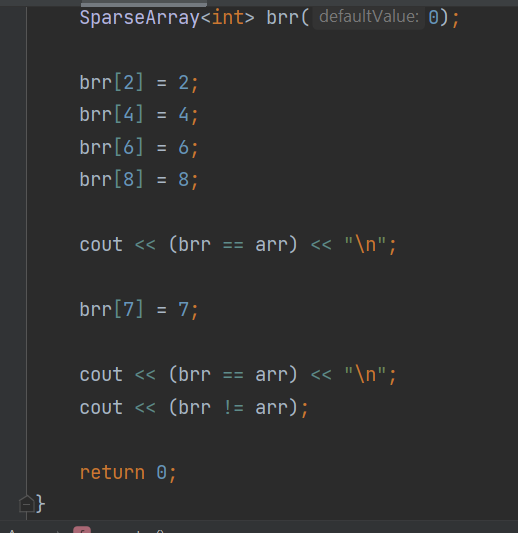
\includegraphics[width=\linewidth]{image.png}
    \caption{Вывод программы}
    \label{fig:my_label}
\end{figure}


\end{document}
